% Options for packages loaded elsewhere
\PassOptionsToPackage{unicode}{hyperref}
\PassOptionsToPackage{hyphens}{url}
\documentclass[
  11pt,
]{article}
\usepackage{xcolor}
\usepackage[margin=22mm]{geometry}
\usepackage{amsmath,amssymb}
\setcounter{secnumdepth}{-\maxdimen} % remove section numbering
\usepackage{iftex}
\ifPDFTeX
  \usepackage[T1]{fontenc}
  \usepackage[utf8]{inputenc}
  \usepackage{textcomp} % provide euro and other symbols
\else % if luatex or xetex
  \usepackage{unicode-math} % this also loads fontspec
  \defaultfontfeatures{Scale=MatchLowercase}
  \defaultfontfeatures[\rmfamily]{Ligatures=TeX,Scale=1}
\fi
\usepackage{lmodern}
\ifPDFTeX\else
  % xetex/luatex font selection
\fi
% Use upquote if available, for straight quotes in verbatim environments
\IfFileExists{upquote.sty}{\usepackage{upquote}}{}
\IfFileExists{microtype.sty}{% use microtype if available
  \usepackage[]{microtype}
  \UseMicrotypeSet[protrusion]{basicmath} % disable protrusion for tt fonts
}{}
\makeatletter
\@ifundefined{KOMAClassName}{% if non-KOMA class
  \IfFileExists{parskip.sty}{%
    \usepackage{parskip}
  }{% else
    \setlength{\parindent}{0pt}
    \setlength{\parskip}{6pt plus 2pt minus 1pt}}
}{% if KOMA class
  \KOMAoptions{parskip=half}}
\makeatother
\usepackage{graphicx}
\makeatletter
\newsavebox\pandoc@box
\newcommand*\pandocbounded[1]{% scales image to fit in text height/width
  \sbox\pandoc@box{#1}%
  \Gscale@div\@tempa{\textheight}{\dimexpr\ht\pandoc@box+\dp\pandoc@box\relax}%
  \Gscale@div\@tempb{\linewidth}{\wd\pandoc@box}%
  \ifdim\@tempb\p@<\@tempa\p@\let\@tempa\@tempb\fi% select the smaller of both
  \ifdim\@tempa\p@<\p@\scalebox{\@tempa}{\usebox\pandoc@box}%
  \else\usebox{\pandoc@box}%
  \fi%
}
% Set default figure placement to htbp
\def\fps@figure{htbp}
\makeatother
\setlength{\emergencystretch}{3em} % prevent overfull lines
\providecommand{\tightlist}{%
  \setlength{\itemsep}{0pt}\setlength{\parskip}{0pt}}
\usepackage{bookmark}
\IfFileExists{xurl.sty}{\usepackage{xurl}}{} % add URL line breaks if available
\urlstyle{same}
\hypersetup{
  hidelinks,
  pdfcreator={LaTeX via pandoc}}

\author{}
\date{}

\begin{document}

\section{Alternation and the index under linear phase
changes}\label{alternation-and-the-index-under-linear-phase-changes}

\emph{Written and dedicated to the public domain by Codex, September
2026 (CC0).}

For matrix symbols, reversing an ordered product is different from
changing the sign of an exterior trace. We first prove the graded trace
identity and expand the full alternating matrix word in the original
phase coordinates. We then follow an actual symbol through an invertible
real linear change, preserving its metric class and exterior inverse,
and determine precisely how its analytic index changes. The result uses
the original matrix index formula with its complete coefficient and
outward orientation.

Read \href{matrix-weyl-index-theorem.pdf}{The matrix Weyl index in the
original phase coordinates} for the all-dimensional theorem (MB10),
\href{scaled-weyl-index-degree.pdf}{Scaled Weyl parametrices and the
surviving differential degree} for the original analytic Fredholm
construction, \href{metric-operator-bounds.pdf}{Metric operator bounds}
for operator-norm continuity, and
\href{relative-projectors-chern-cutoff.pdf}{Relative Weyl projectors and
the Chern cutoff form} for the full matrix exterior and cutoff setting.
\href{ordered-weyl-exterior-reduction.pdf}{From ordered Weyl errors to
the exterior index form}, equations (5)--(18), gives the independent
direct proof from the same ordered errors.

\subsection{1. Ordered exterior products and graded cyclic
trace}\label{ordered-exterior-products-and-graded-cyclic-trace}

Let \(\alpha\) and \(\beta\) be matrix-valued differential forms of
degrees \(p\) and \(q\). Their exterior product wedges scalar form
components and multiplies matrices in the written order. Expanding in
elementary forms and using the finite matrix identity
\(\operatorname{tr}(UV)=\operatorname{tr}(VU)\) gives \[
 \operatorname{Tr}(\alpha\wedge\beta)
       =(-1)^{pq}\operatorname{Tr}(\beta\wedge\alpha).
 \tag{EF1}
\] This is a statement after matrix trace; the untraced products
generally differ. In particular, for one-forms \(\alpha,\beta\), rotate
the first factor of the \(2n\)-fold ordered word
\((\alpha\wedge\beta)^n\) past the remaining \(2n-1\) one-forms. Its
sign is \(-1\), so \[
 \operatorname{Tr}[(\alpha\wedge\beta)^n]
       =-\operatorname{Tr}[(\beta\wedge\alpha)^n].
 \tag{EF2}
\] Taking \(\alpha=db,\beta=da\) proves the trace relation needed for
the two parametrix orders without interchanging any untraced matrix
factors.

To see the full orientation coefficient, put
\(z_{2j-1}=x_j,z_{2j}=\xi_j\) and
\(\Omega=dz_1\wedge\cdots\wedge dz_{2n}\). Directly expanding every
wedge gives \[
 \operatorname{Tr}[(db\wedge da)^n]
 =\left[
 \sum_{\sigma\in S_{2n}}\operatorname{sgn}(\sigma)\,
 \operatorname{tr}\!\left(
   \prod_{r=1}^{n}
    \bigl[(\partial_{z_{\sigma(2r-1)}}b)
          (\partial_{z_{\sigma(2r)}}a)\bigr]\right)
  \right]\Omega .
 \tag{EF3}
\] The product over \(r\) is ordered from \(1\) to \(n\). Every
permutation appears once, with its actual sign; no scalar determinant
replaces the matrix word. For \(n=1\), its coefficient is
\(\operatorname{tr}(b_xa_\xi-b_\xi a_x)\), the negative of the stated
matrix Poisson bracket convention.

The matrix Poisson bracket itself is not generally antisymmetric before
trace: \[
 \{b,a\}
  =\sum_j(b_{\xi_j}a_{x_j}-b_{x_j}a_{\xi_j}),
 \qquad
 \{a,b\}
  =\sum_j(a_{\xi_j}b_{x_j}-a_{x_j}b_{\xi_j}).
 \tag{EF4}
\] For a compactly supported example in dimension one, choose a smooth
cutoff \(\rho\) equal to one near \((0,0)\), \(A=E_{12}\), \(D=E_{21}\),
\(a=\rho xA\), and \(b=\rho\xi D\). At the origin, \(\{b,a\}=DA=E_{22}\)
and \(\{a,b\}=-AD=-E_{11}\). Their sum \(E_{22}-E_{11}\ne0\). This
example proves why the exact alternating \emph{trace of exterior words}
in (EF2) cannot be replaced by pointwise scalar antisymmetry.

\subsection{2. The original isotropic symbol under a fixed linear
map}\label{the-original-isotropic-symbol-under-a-fixed-linear-map}

Keep \(g_z=(1+|z|^2)^{-1}|dz|^2\) on \(\mathbb R^{2n}\) and
\(a\in S(1,g;\operatorname{End}\mathbb C^\nu)\), uniformly invertible
outside a ball. If \(T\in GL(2n,\mathbb R)\), define the actual
transformed symbol \(a_T(z)=a(Tz)\), with no replacement of its matrix
values. For every derivative order \(k\), the linear chain rule writes
\(D^k a_T(z)\) as a finite sum of \(D^k a(Tz)\) applied to \(T\)-images
of the \(k\) directions. Since
\(\langle Tz\rangle\asymp_T\langle z\rangle\), the defining seminorms
give \[
 a_T\in S(1,g),\qquad
 \|D^k a_T(z)\|
       \le C_{T,k}\langle z\rangle^{-k}.
 \tag{LS1}
\] If \(a(w)\) is invertible for \(|w|\ge R\), then \(a_T(z)\) is
invertible for \(|z|\ge\|T^{-1}\|R\), with the same bound on its
pointwise inverse. The proved scaled-parametrix result IP14 therefore
makes \(a_T^w\) Fredholm for every \(T\in GL(2n,\mathbb R)\).

\subsection{3. Norm-continuous transport along one
component}\label{norm-continuous-transport-along-one-component}

Let \(T_t\), \(0\le t\le1\), be a continuously differentiable path in
\(GL(2n,\mathbb R)\). Compactness of the parameter interval supplies
common bounds for \(T_t\), \(T_t^{-1}\) and \(\dot T_t\).
Differentiating any order-\(k\) spatial derivative of \(a(T_tz)\)
produces terms with \(D^k a(T_tz)\) times one differentiated \(T_t\)
factor, and a term with \(D^{k+1}a(T_tz)\dot T_tz\). The latter is
bounded by \(C\langle z\rangle^{-k-1}|z|\), so every term obeys the
original \(S(1,g)\) order-\(k\) bound uniformly in \(t\). The
fundamental theorem of calculus therefore gives convergence in each
fixed finite symbol seminorm as \(t\) varies. B26 turns this into
operator-norm continuity: \[
 t\longmapsto(a\circ T_t)^w
       \quad\text{is continuous in }
       \mathcal L(L^2(\mathbb R^n;\mathbb C^\nu)).
 \tag{LS2}
\] Every member is Fredholm by Section 2. Norm stability of the Fredholm
index gives \[
 \operatorname{ind}(a\circ T_1)^w
       =\operatorname{ind}(a\circ T_0)^w .
 \tag{LS3}
\]

For clarity, the component with positive determinant is path connected
without invoking an index theorem. Write \(T=QP\) with
\(P=(T^tT)^{1/2}\) positive definite and \(Q=TP^{-1}\in SO(2n)\). The
path \((1-s)I+sP\) stays positive definite. Every real special
orthogonal matrix has an orthogonal decomposition into two-dimensional
rotation planes and fixed \(+1\) directions: complex nonreal eigenvalues
occur in conjugate pairs, while the \(-1\) eigenspace has even dimension
because the determinant is \(+1\), and can be paired into rotation
planes of angle \(\pi\). Decreasing each rotation angle continuously to
zero gives a path in \(SO(2n)\) from \(Q\) to \(I\). Concatenating these
paths yields a path from \(I\) to \(T\) in \(GL^+(2n,\mathbb R)\). Hence
\[
 \det T>0
 \quad\Longrightarrow\quad
 \operatorname{ind}(a\circ T)^w
       =\operatorname{ind}a^w .
 \tag{LS4}
\] This proves the positive-determinant half of the analytic assertion
independently of any exterior formula.

\subsection{4. The boundary functional under both determinant
signs}\label{the-boundary-functional-under-both-determinant-signs}

On the invertibility region let \(\theta_a=a^{-1}da\). The ordinary
pullback chain rule retains the matrix factor order and gives \[
 (a\circ T)^{-1}d(a\circ T)=T^*\theta_a,\qquad
 \operatorname{Tr}
   [((a\circ T)^{-1}d(a\circ T))^{2n-1}]
   =T^*\operatorname{Tr}(\theta_a^{2n-1}).
 \tag{LS5}
\] The closed odd trace form used for the boundary comparison has a
complete local proof. On the original invertibility region differentiate
\(a^{-1}a=I\). This gives \(d(a^{-1})=-a^{-1}(da)a^{-1}\), so \[
 d\theta_a=-\theta_a^2,\qquad
 d(\theta_a^{\,2n-1})
 =-\sum_{r=0}^{2n-2}(-1)^r\theta_a^{\,2n}
 =-\theta_a^{\,2n}.                                      \tag{EF5}
\] The sum has \(2n-1\) terms and its alternating sum is one. By EF1,
rotating the first degree-one factor of the even word gives
\(\operatorname{Tr}(\theta_a^{2n})=-\operatorname{Tr}(\theta_a^{2n})\),
hence \[
 d\,\operatorname{Tr}(\theta_a^{\,2n-1})
 =-\operatorname{Tr}(\theta_a^{\,2n})=0.                   \tag{EF6}
\] Every matrix multiplication and differential form remains in its
original order before taking the graded trace.

Choose a ball \(B_R\) in the \(z\) variables large enough that both its
boundary and the boundary of \(T(B_R)\) lie in the respective
invertibility regions and \(T(B_R)\) contains the original noninvertible
compact set. Orient every boundary by the stipulated positive ambient
form \(\Omega=dx_1\wedge d\xi_1\wedge\cdots\wedge dx_n\wedge d\xi_n\).
The boundary change-of-variables rule, obtained by applying the Jacobian
sign to an outward-normal-first oriented frame, gives \[
 \int_{\partial B_R}
       T^*\operatorname{Tr}(\theta_a^{2n-1})
 =\operatorname{sgn}(\det T)
       \int_{\partial T(B_R)}
             \operatorname{Tr}(\theta_a^{2n-1}).
 \tag{LS6}
\] EF6 proves this odd trace form is closed on the invertibility region.
Apply Stokes to the region between \(\partial T(B_R)\) and any
sufficiently large enclosing sphere \(\partial B_{R'}\); the outer and
inner induced boundary orientations have opposite signs. Therefore the
two integrals without the Jacobian factor agree. In particular the
original boundary functional obeys \[
 \int_{\partial B_R}
   \operatorname{Tr}
     [((a\circ T)^{-1}d(a\circ T))^{2n-1}]
 =\operatorname{sgn}(\det T)
       \int_{\partial B_{R'}}
             \operatorname{Tr}[(a^{-1}da)^{2n-1}] .
 \tag{LS7}
\] This is an exact geometric sign statement for every dimension. It
does not rely on equality between the boundary functional and the
analytic index.

\subsection{5. Direct checks in dimensions one and
two}\label{direct-checks-in-dimensions-one-and-two}

For \(n=1\), equations (16), (18) and (19) of
\href{ordered-weyl-exterior-reduction.pdf}{From ordered Weyl errors to
the exterior index form} directly prove the full analytic formula with
the original \(dx_1\wedge d\xi_1\) orientation:
\(\operatorname{ind}a^w=(2\pi i)^{-1}
\int_{\partial B}\operatorname{Tr}(a^{-1}da)\). Apply that same proved
formula to \(a\circ T\), then use (LS7). This gives, for every
\(T\in GL(2,\mathbb R)\), \[
 \operatorname{ind}(a\circ T)^w
   =\operatorname{sgn}(\det T)\operatorname{ind}a^w
       \qquad(n=1).
 \tag{LS8}
\] For \(n=2\), equations (16), (18), (20) and (21) of that same direct
lesson evaluate the finite coefficient completely, with the original
ambient orientation and the same analytic receiving map for \(a\) and
\(a\circ T\). Apply that proved formula to both symbols, and then apply
(LS7) to their odd boundary forms. The exact constant \(1/(24\pi^2)\) is
identical on both sides, so it factors out without a sign change. Thus
\[
 \operatorname{ind}(a\circ T)^w
    =\operatorname{sgn}(\det T)\operatorname{ind}a^w
       \qquad(T\in GL(4,\mathbb R),\ n=2).
 \tag{LS9}
\] The dimension-one and dimension-two calculations independently check
the all-dimensional argument that follows.

\subsection{6. The all-dimensional analytic
sign}\label{the-all-dimensional-analytic-sign}

MB10 proves for every \(n\geq1\), every original
\(a\in S(1,g;\operatorname{End}\mathbb C^\nu)\) uniformly invertible
outside a compact set, and the original \(\Omega\)-outward boundary
orientation, \[
 \operatorname{ind}a^w
 =D_n\int_{\partial B}^{\Omega}
       \operatorname{Tr}[(a^{-1}da)^{2n-1}],
 \qquad
 D_n=-(-2\pi i)^{-n}
                 \frac{(n-1)!}{(2n-1)!}.
 \tag{LS10}
\] This is the full coefficient, with its sign, \(\pi\)- and
\(i\)-powers and factorials. LS1 proves that \(a\circ T\) meets the
\textbf{same} symbol and exterior-invertibility hypotheses for every
\(T\in GL(2n,\mathbb R)\); its matrix size and its \(D_n\) are
unchanged. Apply (LS10) to \(a\circ T\), use the exact pullback identity
(LS5) and the oriented boundary change (LS7), and then apply (LS10) back
to \(a\): \[
\begin{aligned}
 \operatorname{ind}(a\circ T)^w
 &=D_n\int_{\partial B_R}^{\Omega}
       \operatorname{Tr}
       [((a\circ T)^{-1}d(a\circ T))^{2n-1}]\\
 &=\operatorname{sgn}(\det T)\,D_n
       \int_{\partial B_{R'}}^{\Omega}
          \operatorname{Tr}[(a^{-1}da)^{2n-1}]\\
 &=\operatorname{sgn}(\det T)\operatorname{ind}a^w,
 \qquad T\in GL(2n,\mathbb R),\quad n,\nu\geq1.
\end{aligned}
\tag{LS11}
\] There is no metaplectic or unitary-conjugacy assertion for a general
\(T\); the second line is the proved boundary pullback, and the first
and last lines are separate applications of the proved original matrix
index theorem. The analytic formula is therefore closed at precisely the
hypotheses of MB10. The independent direct calculation in the
exterior-reduction lesson, equations (5)--(18), proves the same analytic
sign using the full finite ordered coefficient and its exterior
evaluation.

\subsection{7. Worked example: a reflection changes a nonzero
index}\label{worked-example-a-reflection-changes-a-nonzero-index}

Use the same full bounded one-plane symbol as (MI1), \[
 a(x,\xi)=\frac{x+i\xi}{\sqrt{1+x^2+\xi^2}},
 \qquad
 T(x,\xi)=(-x,\xi),\qquad \det T=-1.
 \tag{LI1}
\] The symbol \(a\) has index \(+1\) by the proved formula (MB10), as
calculated directly in (MI2). Both \(a\) and \(a\circ T\) belong to the
original \(S(1,g)\) class and have a uniformly bounded inverse outside a
ball. On the positively oriented circle
\((x,\xi)=R(\cos\vartheta,\sin\vartheta)\), the denominator is positive
and \[
 (a\circ T)(R\cos\vartheta,R\sin\vartheta)
   =\frac{R e^{i(\pi-\vartheta)}}{\sqrt{1+R^2}},
 \qquad
 (a\circ T)^{-1}d(a\circ T)=-i\,d\vartheta.
 \tag{LI2}
\] The original \(n=1\) coefficient is \(D_1=1/(2\pi i)\). Therefore \[
 \operatorname{ind}(a\circ T)^w
 =\frac1{2\pi i}\int_0^{2\pi}(-i)\,d\vartheta
 =-1
 =\operatorname{sgn}(\det T)\operatorname{ind}a^w.
 \tag{LI3}
\] This checks an actual nonzero analytic sign change without treating
the non-symplectic reflection as a unitary conjugation.

\subsection{8. Exercises with solutions}\label{exercises-with-solutions}

\textbf{Exercise 1.} In two phase planes let \(T\) change only \(x_1\)
to \(-x_1\), leaving \(\xi_1,x_2,\xi_2\) fixed. Determine the index of
\((a\circ T)^w\) from \(\operatorname{ind}a^w=m\), and calculate the
coefficient \(D_2\) separately.

\textbf{Solution.} In the original ordered coordinates \(\det T=-1\).
Equation (LS11) gives \(\operatorname{ind}(a\circ T)^w=-m\), including
for noncommutative matrix symbols. The complete coefficient is \[
 D_2=-(-2\pi i)^{-2}\frac{1!}{3!}
     =\frac{1}{24\pi^2}.
 \tag{LI4}
\] The minus sign of the transformed index comes from the boundary
orientation in (LS7), not from changing \(D_2\).

\textbf{Exercise 2.} Why does
\(\operatorname{Tr}[(db\wedge da)^n]=-\operatorname{Tr}[(da\wedge db)^n]\)
not imply \(\{b,a\}=-\{a,b\}\) as untraced matrices?

\textbf{Solution.} Equation (EF2) rotates one degree-one factor through
\(2n-1\) others \textbf{inside a matrix trace}, using graded cyclicity
(EF1). It does not commute the matrix coefficients. In (EF4)'s exact
compact two-by-two local example, \(\{b,a\}=E_{22}\) and
\(\{a,b\}=-E_{11}\) at the origin, so their untraced sum
\(E_{22}-E_{11}\) is nonzero. The traced exterior assertion and the
untraced Poisson assertion have different algebraic hypotheses.

\subsection{9. References}\label{references}

\begin{itemize}
\tightlist
\item
  M. Pflaum, H. Posthuma and X. Tang, \emph{Cyclic cocycles on
  deformation quantizations and higher index theorems},
  \href{https://arxiv.org/abs/0805.1411}{arXiv:0805.1411v3},
  IndThms.tex, theorem thm:higher-algind and proof, lines 412--479. The
  preceding matrix-index lesson proves its specialization to the
  original symbols and all factor and orientation comparisons.
\end{itemize}

\subsection{10. Every derivative in the linear
transport}\label{every-derivative-in-the-linear-transport}

Here we supply the estimates and finite-dimensional constructions used
in Sections 2--4. Keep the original ordered coordinates, the full matrix
symbol and the actual map \(T\). Write \(d=2n\),
\(\langle z\rangle=(1+|z|^2)^{1/2}\), and, for this same symbol, set \[
 A_k(a)=\sup_z\langle z\rangle^k
       \|D^k a(z)\|_{(\mathbb R^d)^k\to\operatorname{End}\mathbb C^\nu},
 \qquad p_{\le J}(a)=\sum_{k=0}^J A_k(a).
 \tag{LT1}
\] For \(k=0\) the norm means the matrix norm itself. These are exactly
the derivative norms for the original metric: \(g_z(v)\le1\) means
\(|v|\le\langle z\rangle\), so the supremum of
\(\|D^ka(z)(v_1,\ldots,v_k)\|\) over the original metric unit vectors is
\(\langle z\rangle^k\|D^ka(z)\|\). They measure the unchanged \(a\); no
coordinate or symbol is being substituted for it. In particular each
\(A_k(a)\) is finite.

Let \[
 m_T=\|T^{-1}\|^{-1},\qquad
 \mu_T=\min(1,m_T),\qquad L_T=\max(1,\|T\|).
 \tag{LT2}
\] The inverse identity gives \(|z|=|T^{-1}Tz|\le\|T^{-1}\||Tz|\), and
the operator norm gives the upper bound. Adding the unchanged constant
one proves both inequalities \[
 \mu_T^2(1+|z|^2)\le1+|Tz|^2
                 \le L_T^2(1+|z|^2).
 \tag{LT3}
\] The complete coordinate chain rule is \[
 \partial_{j_1}\cdots\partial_{j_k}a(Tz)
 =\sum_{\ell_1,\ldots,\ell_k=1}^d
       \left(\prod_{r=1}^k T_{\ell_rj_r}\right)
       (\partial_{\ell_1}\cdots\partial_{\ell_k}a)(Tz).
 \tag{LT4}
\] The product here consists of scalar entries; the matrix derivative
remains intact. For \(k=0\) the sum has its single empty term \(a(Tz)\).
The first-order formula follows by differentiating each coordinate of
\(Tz\). Induction differentiates only the last derivative, because every
entry of \(T\) is constant in \(z\), and proves the displayed sum for
every \(k\).

Equivalently, applying that full sum to \(v_1,\ldots,v_k\) gives
\(D^ka(Tz)(Tv_1,\ldots,Tv_k)\). Hence \[
 A_k(a\circ T)\le\|T\|^k\mu_T^{-k}A_k(a).
 \tag{LT5}
\] All constants and the original \(1+|z|^2\) are retained in
(LT3)--(LT5). If coordinate derivative norms are used instead, expanding
the same multilinear form gives their comparison explicitly. With
\(M_k\) the maximum of the weighted norms of its coordinate derivatives,
\[
 M_k(a)\le A_k(a)\le d^{k/2}M_k(a).
 \tag{LT6}
\] Indeed the expansion has all \(d^k\) terms, and its norm is bounded
by \(M_k\prod_r\sum_j|v_{rj}|\). Cauchy--Schwarz gives
\(\sum_j|v_{rj}|\le\sqrt d\,|v_r|\). The other inequality evaluates the
multilinear form on coordinate unit vectors. Thus either of these finite
seminorm lists gives the exact continuity required by B26.

Now let \(T_t\) be the original continuously differentiable path. The
full derivative of (LT4), including every matrix-entry derivative and
every coordinate of \(\dot T_tz\), is \[
\begin{aligned}
 &\partial_t\partial_{j_1}\cdots\partial_{j_k}a(T_tz)\\
 &=\sum_{\ell_1,\ldots,\ell_k=1}^d
   \sum_{s=1}^k
       (\dot T_t)_{\ell_sj_s}
       \left(\prod_{\substack{1\le r\le k\\r\ne s}}
                    (T_t)_{\ell_rj_r}\right)
       (\partial_{\ell_1}\cdots\partial_{\ell_k}a)(T_tz)\\
 &\quad+\sum_{\ell_1,\ldots,\ell_k=1}^d
       \left(\prod_{r=1}^k(T_t)_{\ell_rj_r}\right)
       \sum_{q,p=1}^d(\dot T_t)_{qp}z_p
       (\partial_q\partial_{\ell_1}\cdots\partial_{\ell_k}a)(T_tz).
\end{aligned}
 \tag{LT7}
\] For \(k=0\) the first sum is empty, and the second is
\(\sum_{q,p}(\dot T_t)_{qp}z_p\partial_qa(T_tz)\). This accounts for the
term that would be lost by differentiating only the prefactor.

Put \(L=\sup_t\|T_t\|\), \(H=\sup_t\|\dot T_t\|\), and
\(\mu=\min(1,\inf_t\|T_t^{-1}\|^{-1})\). The inverse entries are the
signed minor polynomials divided by the nonzero determinant; they are
continuous. On the compact interval the norms are bounded, so \(L>0\),
\(H<\infty\) and \(\mu>0\). In multilinear notation the first sum in
(LT7) has \(k\) terms with one \(\dot T_t\) and \(k-1\) copies of
\(T_t\). The second has \(k\) copies of \(T_t\) and the extra argument
\(\dot T_tz\). Using (LT3) for this common \(\mu\) yields \[
 A_k\bigl(\partial_t(a\circ T_t)\bigr)
 \le H\left[kL^{k-1}\mu^{-k}A_k(a)
                 +L^k\mu^{-k-1}A_{k+1}(a)\right].
 \tag{LT8}
\] At \(k=0\) omit the first term. In the last term the retained factor
is \(|z|/\langle z\rangle\le1\). The finite-dimensional fundamental
theorem of calculus, applied to every matrix entry and derivative, gives
\[
 A_k(a\circ T_t-a\circ T_u)
 \le |t-u|H\left[kL^{k-1}\mu^{-k}A_k(a)
                 +L^k\mu^{-k-1}A_{k+1}(a)\right].
 \tag{LT9}
\] The common bound permits the supremum in \(z\) and unit directions
after integration. Summing through the actual finite \(J\) of B26 proves
(LS2), with every spatial derivative and parameter derivative accounted
for.

There is a stronger continuity statement. Fix \(T\in GL(d,\mathbb R)\)
and take \(S\) with \(\|S-T\|<m_T/2\). Along the actual segment
\(T_s=T+s(S-T)\), \[
 |T_sz|\ge(m_T-\|S-T\|)|z|\ge(m_T/2)|z|,
 \qquad\|T_s\|\le\|T\|+m_T/2.
 \tag{LT10}
\] The lower bound makes every \(T_s\) injective, hence invertible in
this finite dimension. Use \(\mu=\min(1,m_T/2)\), \(L=\|T\|+m_T/2\) and
\(H=\|S-T\|\) in (LT9). It proves \[
 A_k(a\circ S-a\circ T)
 \le\|S-T\|\left[kL^{k-1}\mu^{-k}A_k(a)
                 +L^k\mu^{-k-1}A_{k+1}(a)\right].
 \tag{LT11}
\] Thus \(T\mapsto a\circ T\) is locally Lipschitz in every fixed
original symbol seminorm. B26 proves local Lipschitz continuity of
\(T\mapsto(a\circ T)^w\) in operator norm. Every \textbf{continuous}
path \(T_t\) consequently gives a continuous operator path;
differentiability of the path is unnecessary. Section 2 and IP14 still
prove Fredholmness at every parameter. The norm-stability proof in
Section 3 of \href{fredholm-stability.pdf}{Finite defects under
perturbation} makes its index locally constant. A locally constant
integer on \([0,1]\) is constant: if two values occurred, the set of
points reached from zero with its value and its open complement would
separate the interval; taking the supremum of an initial interval of
that value contradicts local constancy at its endpoint. This proves
(LS3) for all continuous paths, while retaining the original
differentiable-path calculation (LT7)--(LT9).

\subsection{11. The full positive square root and orthogonal rotation
planes}\label{the-full-positive-square-root-and-orthogonal-rotation-planes}

We prove the original polar and orthogonal-plane assertions. First
consider any real symmetric \(d\)-by-\(d\) matrix \(H\). Its quadratic
form has a maximum on the unit sphere. Here is the finite compactness
fact needed for this statement. A bounded real sequence has a convergent
subsequence: bisect a containing closed interval, keep a half containing
infinitely many terms, repeat, and choose increasing sequence indices
from those halves. The nested lengths tend to zero; the chosen values
converge to their common endpoint limit. Repeating for each of the
finitely many coordinates yields a convergent subsequence of any bounded
sequence in \(\mathbb R^d\). The unit sphere is closed because the sum
of coordinate squares is continuous. A maximizing sequence for the
bounded continuous quadratic form therefore has a sphere subsequence
whose limit attains its supremum. Its boundedness follows from the
finite sum \(\sum_{j,k}|H_{jk}||v_j||v_k|\) for \(|v|=1\).

Let \(v\) be such a maximizing unit vector and \(u\perp v\). On the unit
curve \((v+tu)/(1+t^2|u|^2)^{1/2}\), the derivative of the quadratic
form at zero is \(2\langle u,Hv\rangle\); it must vanish. Thus
\(Hv=\lambda v\). Symmetry gives
\(\langle v,Hu\rangle=\langle Hv,u\rangle=0\), so \(v^\perp\) is
invariant. Induction on its dimension gives an orthonormal eigenbasis
\(v_1,\ldots,v_d\), with \[
 H=\sum_{j=1}^d\lambda_j v_jv_j^t.
 \tag{LP1}
\] All eigenvalues and all orthogonal projections are retained. For the
original \(H=T^tT\), \[
 \lambda_j=\langle v_j,T^tTv_j\rangle=|Tv_j|^2>0,
 \qquad
 P=\sum_{j=1}^d\sqrt{\lambda_j}\,v_jv_j^t,
 \quad
 P^{-1}=\sum_{j=1}^d\lambda_j^{-1/2}v_jv_j^t.
 \tag{LP2}
\] Orthogonality of the projections proves \(P^2=T^tT\), \(PP^{-1}=I\),
and positive definiteness of \(P\). This positive symmetric square root
is unique. If \(W\) is another such root, then \(WH=HW\), since
\(H=W^2\); it preserves each eigenspace of \(H\). Apply (LP1) to its
symmetric restriction there. Every positive eigenvalue \(r\) of \(W\)
satisfies \(r^2=\lambda\), so that restriction is \(\sqrt\lambda I\).
Hence \(W=P\).

Set \(Q=TP^{-1}\), exactly as in Section 3. Direct multiplication proves
\[
 Q^tQ=P^{-1}T^tTP^{-1}=I,
 \qquad T=QP,
 \qquad
 \det P=\prod_{j=1}^d\sqrt{\lambda_j}>0,
 \qquad\det Q=\frac{\det T}{\prod_j\sqrt{\lambda_j}}.
 \tag{LP3}
\] An orthogonal matrix has determinant \(+1\) or \(-1\), since taking
determinants in \(Q^tQ=I\) gives \((\det Q)^2=1\). Thus its determinant
is precisely the sign of the original \(\det T\). The original
positive-definite path also follows without deleting any eigenspace: \[
 (1-s)I+sP
       =\sum_{j=1}^d(1-s+s\sqrt{\lambda_j})v_jv_j^t,
 \qquad 0\le s\le1.
 \tag{LP4}
\] Every coefficient is positive, including at both endpoints.

For the rotation-plane assertion, start with this same real orthogonal
\(Q\) and retain both its parts \[
 C=\tfrac12(Q+Q^t),\qquad K=\tfrac12(Q-Q^t),
 \qquad C^t=C,\quad K^t=-K.
 \tag{LP5}
\] Since \(QQ^t=Q^tQ=I\), expanding both products gives \[
 CK=KC,\qquad C^2-K^2=I,
 \qquad Q=C+K.
 \tag{LP6}
\] By (LP1), \(C\) has mutually orthogonal real eigenspaces \(E_c\).
Commutation shows \(K(E_c)\subset E_c\). On that actual space, \[
 K^2=(c^2-1)I,
 \qquad |Kv|^2=-\langle v,K^2v\rangle=(1-c^2)|v|^2.
 \tag{LP7}
\] Therefore \(|c|\le1\). If \(c=1\) or \(c=-1\), the right side is
zero, so \(K=0\) there and \(Q=I\) or \(Q=-I\), respectively. If
\(-1<c<1\), put \(\sigma=(1-c^2)^{1/2}>0\). Choose a unit \(v\in E_c\)
and put \(w=Kv/\sigma\). Skew symmetry gives \(\langle v,w\rangle=0\);
(LP7) gives \(|w|=1\). The full action on this plane is \[
 Kv=\sigma w,\quad Kw=-\sigma v,
 \qquad
 Qv=cv+\sigma w,\quad Qw=-\sigma v+cw.
 \tag{LP8}
\] Its orthogonal complement inside \(E_c\) is invariant under \(K\),
because inner products of \(Ku\) with \(v,w\) equal the negatives of the
inner products of \(u\) with \(Kv,Kw\). Repeating decomposes all of
\(E_c\) into these two-dimensional planes. Each plane has the exact
matrix \[
 R(c,\sigma)=\begin{pmatrix}c&-\sigma\\\sigma&c\end{pmatrix},
 \qquad c^2+\sigma^2=1,\quad\det R=1.
 \tag{LP9}
\] The remaining spaces are fixed \(+1\) directions and \(-1\)
directions. The determinant of \(Q\) is the product of their signs and
the plane determinants. When \(\det Q=1\), the number of \(-1\)
directions is even, and pairing them gives planes \(R(-1,0)\). This
proves the exact decomposition claimed earlier. Its complex eigenvalues
on each nonreal plane are the conjugate roots \(c+i\sigma,c-i\sigma\) of
\(\lambda^2-2c\lambda+1\); the \(-1\) and \(+1\) cases were proved over
the reals as well.

We also construct every needed path explicitly. If
\((c,\sigma)\ne(-1,0)\), define \[
 (c_s,\sigma_s)=
 \frac{(1-s+sc,\,s\sigma)}
      {\sqrt{(1-s+sc)^2+s^2\sigma^2}},\qquad 0\le s\le1.
 \tag{LP10}
\] The denominator can vanish only if \(s\sigma=0\) and \(1-s+sc=0\). At
\(s=0\) the second expression is one. If \(s>0\), these two equalities
force \(\sigma=0,c=-1,s=1/2\), which was excluded. Thus (LP10) is a
smooth path of actual unit pairs from \((1,0)\) to \((c,\sigma)\). For
\((-1,0)\), use first the same normalized segment from \((1,0)\) to
\((0,1)\), then the segment from \((0,1)\) to \((-1,0)\). Neither
segment has opposite endpoints, so the same nonvanishing proof applies.
Every matrix \(R(c_s,\sigma_s)\) is real orthogonal with determinant
one.

Choose the actual orthonormal basis of all these planes and fixed
directions, and call its change-of-basis matrix \(O\). Conjugating the
block paths by \(O\) gives a continuous, piecewise smooth
\(Q_s\in SO(d)\) with \(Q_0=I,Q_1=Q\). No eigenvalue, direction or plane
is discarded. The exact concatenated path from the identity to the
original \(T\) is \[
 T_s=\begin{cases}
       Q_{2s},&0\le s\le\tfrac12,\\
       Q\bigl((2-2s)I+(2s-1)P\bigr),&\tfrac12\le s\le1.
      \end{cases}
 \tag{LP11}
\] Its endpoints are \(I,T\), the two formulas agree at \(s=1/2\), and
their determinants are positive by (LP4) and \(\det Q=1\). Equations
(LT10)--(LT11) and Fredholm stability apply to this continuous path,
proving (LS4) with all its prerequisites supplied.

For completeness these are exactly the two path components of
\(GL(d,\mathbb R)\). A continuous determinant cannot pass between its
signs without zero, by the intermediate value theorem. The positive
component is connected by (LP11). For a negative-determinant \(T\),
retain \(J=\operatorname{diag}(-1,1,\ldots,1)\). The matrix \(JT\) has
positive determinant; multiplying its identity-to-\(JT\) path on the
left by this same \(J\) gives a negative-determinant path from \(J\) to
\(T\). This proves connectedness of that component. The analytic index
of \((a\circ T)^w\) is consequently constant on each component for the
unchanged \(a\), by (LS3).

\subsection{12. The oriented boundary comparison with a global
primitive}\label{the-oriented-boundary-comparison-with-a-global-primitive}

We give the complete integration argument for (LS6)--(LS7). It also
proves a geometric strengthening: these two boundary identities hold for
any smooth \(\nu\)-by-\(\nu\) matrix \(a\) on \(\mathbb R^{2n}\) that is
invertible outside a compact set. Neither symbol estimates nor a uniform
bound on the exterior inverse is needed for this geometric assertion.
The analytic Fredholm results continue to use their original symbol and
inverse bounds.

Choose \(\rho>0\) so that the noninvertible set lies in \(B_\rho\). A
smooth admissible cutoff can be constructed explicitly. Set
\(\eta(t)=e^{-1/t}\) for \(t>0\) and \(\eta(t)=0\) for \(t\le0\), and \[
 \chi(t)=\frac{\eta(t)}{\eta(t)+\eta(1-t)},\qquad
 \psi(z)=\chi\!\left(\frac{|z|^2-\rho^2}{3\rho^2}\right).
 \tag{LG1}
\] Every derivative of \(\eta\) on \(t>0\) is \(e^{-1/t}\) times a
finite polynomial in \(t^{-1}\). Each tends to zero at the origin: with
\(u=1/t\), the inequality \(e^u\ge u^N/N!\), taking \(N\) greater than
each polynomial degree, proves this limit. Induction therefore proves
that the zero extension is smooth. The denominator in \(\chi\) is
positive everywhere, since \(t\le0\) and \(1-t\le0\) cannot both hold.
Thus \(\psi\) is smooth, is zero on \(\overline{B_\rho}\), and is one
for \(|z|\ge2\rho\). In particular
\(K=\operatorname{supp}(1-\psi)=\overline{B_{2\rho}}\), and every
possible noninvertible point has a neighborhood where \(\psi=0\).

On the actual invertibility region \(U_a\), keep \[
 \theta=a^{-1}da,\quad\omega=\operatorname{Tr}(\theta^{2n-1}),
 \qquad
 F_n(t)=n\int_0^t u^{n-1}(1-u)^n\,du
       =n\sum_{j=0}^n(-1)^j\binom nj\frac{t^{n+j}}{n+j}.
 \tag{LG2}
\] Equations (EF1), (EF5) and (EF6) prove \(d\omega=0\), with all matrix
orders retained. Define \(\beta=F_n(\psi)\omega\) on \(U_a\), extending
it by zero near the noninvertible set. It is globally smooth:
\(F_n(0)=0\), and \(\psi\) is identically zero on that whole
neighborhood. The complete product differentiation gives \[
 \begin{aligned}
 d\beta
 &=n\psi^{n-1}(1-\psi)^n d\psi\wedge\omega
                         +F_n(\psi)d\omega\\
 &=n\psi^{n-1}(1-\psi)^n d\psi\wedge\omega,\\
 F_n(1)&=n\int_0^1u^{n-1}(1-u)^n\,du
           =\frac{n\,(n-1)!\,n!}{(2n)!}
           =\frac{(n!)^2}{(2n)!}>0.
 \end{aligned}
 \tag{LG3}
\] The first term extends by zero in the same manner. Its support is
contained in the original compact \(K\), since \(d\psi=0\) where
\(\psi=1\). The full factorial moment is proved by repeated
one-dimensional integration by parts in ES4 of
\href{relative-projectors-chern-cutoff.pdf}{Relative Weyl projectors and
the Chern cutoff form}. Its positivity also follows directly from its
strictly positive integrand on \(0<u<1\). Equation (LG3) is the same
global primitive as BN2--BN3, with all its factors intact.

We first justify the exact distinction between the signed determinant
and the absolute determinant in integration. For any compactly supported
smooth complex function \(f\) on \(\mathbb R^d\) and any real invertible
\(T\), \[
 \int_{\mathbb R^d}f(Tz)\,dz
       =\frac1{|\det T|}\int_{\mathbb R^d}f(w)\,dw,
 \qquad T^*\Omega=(\det T)\Omega.
 \tag{LG4}
\] For the first equality it suffices to prove it for the exact
elementary factors of \(T\). Swapping two coordinates preserves the
Lebesgue integral by Fubini and has determinant \(-1\). Scaling one
coordinate by \(c\ne0\) gives the factor \(1/|c|\) by the
one-dimensional substitution formula; when \(c<0\), reversing the
integration endpoints supplies the absolute value. Adding \(c\) times
coordinate \(k\) to a different coordinate \(j\) preserves the integral:
fix every other coordinate and translate the \(j\)-th line by the actual
constant \(cz_k\). Its determinant is one. The one-dimensional
substitutions follow from the fundamental theorem of calculus applied to
a compactly supported continuous integrand's primitive. All the
functions here are integrable, so Fubini applies to their real and
imaginary parts.

Every invertible matrix is a finite product of these actual elementary
factors. At each elimination stage its next column has a nonzero entry
among the remaining rows; otherwise the remaining square block would
have a zero column and determinant zero. Swap that entry into the pivot
position, scale by its nonzero pivot inverse, and subtract its required
multiples from the other rows. Continuing in the remaining block and
then eliminating above the pivots produces the identity. Each reverse
step is an elementary factor of the same type. Their determinants
multiply, so applying their already proved substitutions successively
gives the full \(|\det T|^{-1}\) in (LG4). This is a proof concerning
the original \(T\), preserving its determinant and all its factors. The
second equality in (LG4) follows by expanding the entire wedge
\(d(Tz)_1\wedge\cdots\wedge d(Tz)_d\): its coefficient is the full
signed permutation sum defining \(\det T\).

Let \(\nu=z/R\) be the unit outward normal to \(\partial B_R\), and set
\(w=Tz\). The ellipsoid \(T(B_R)\) is defined by \(|T^{-1}w|^2<R^2\).
Differentiating this full quadratic defining function gives its unit
outward normal and the full transverse factor \[
 \nu_w=\frac{T^{-t}\nu}{|T^{-t}\nu|},\qquad
 (T\nu)\cdot\nu_w=\frac1{|T^{-t}\nu|}>0.
 \tag{LG5}
\] Thus \(T\nu\) is outward transverse, even though it generally differs
from the Euclidean normal. If \((e_1,\ldots,e_{d-1})\) is a positive
orthonormal tangent frame on the sphere, then the complete determinant
identity gives \[
 \Omega(T\nu,Te_1,\ldots,Te_{d-1})=\det T,
 \qquad
 \Omega(\nu_w,Te_1,\ldots,Te_{d-1})
                      =|T^{-t}\nu|\det T.
 \tag{LG6}
\] To obtain the second equality, subtract from \(T\nu\) its tangent
component; wedge evaluation kills that component, while its remaining
normal component is exactly (LG5). The absolute value of the second
determinant is the tangential area factor \[
 J_{\partial T}(z)=|\det T|\,|T^{-t}\nu|.
 \tag{LG7}
\] Indeed the squared volume of a tangent parallelepiped equals its Gram
determinant, by expanding its coordinates in any orthonormal basis of
the tangent hyperplane. Adjoining the unit normal does not change that
Gram determinant. This proves the area factor and the orientation sign
simultaneously: the actual image tangent frame is positive precisely
when \(\det T>0\).

These frame identities prove the boundary substitution for any smooth
\((d-1)\)-form \(\gamma\) on a neighborhood of the ellipsoid boundary.
Use the finite sphere graph charts from the proof of ES6--ES7 in the
relative-projector lesson. In a chart \(z=z(u)\), the image chart is
exactly \(w=Tz(u)\), and pullback evaluation is
\(\gamma_w(T\partial_{u_1}z,\ldots,T\partial_{u_{d-1}}z)\). The image
area is multiplied by (LG7); its orientation relative to the outward
image normal has the sign given by (LG6). Integrating each chart, with a
partition of unity transported by \(T\), therefore proves \[
 \int_{\partial B_R}^{\Omega}T^*\gamma
       =\frac{\det T}{|\det T|}
           \int_{\partial T(B_R)}^{\Omega}\gamma.
 \tag{LG8}
\] There is no unstated sign from a normal replacement: its multiplier
was proved positive in (LG5). A finite partition can be constructed by
choosing smaller graph neighborhoods covering the compact sphere, taking
smooth nonnegative coordinate cutoffs positive on those smaller
neighborhoods, and dividing each by the positive sum. Coordinate cutoffs
follow from the same \(\eta\) construction in (LG1). Their transported
sum is still one. Thus the chart sums give the full boundaries,
including the overlaps. Applying (LG8) to \(\gamma=\omega\) proves
(LS6).

Finally choose actual radii \[
 R>2\rho\max(1,\|T^{-1}\|),\qquad
 R'>\max(2\rho,\|T\|R).
 \tag{LG9}
\] Then \(K\subset B_R\), \(K\subset T(B_R)\), and
\(T(B_R)\subset B_{R'}\), with collars of all relevant boundaries lying
where \(\psi=1\). Write the globally smooth compact derivative as
\(d\beta=V(w)\Omega\). Its pullback is the full top form
\(T^*d\beta=(\det T)V(Tz)\Omega\). The supports of \(V\) and
\(V\circ T\) are inside \(B_{R'}\) and \(B_R\), respectively. Applying
(LG4) to this actual compact \(V\), with no interior inverse required,
proves \[
\begin{aligned}
 \int_{B_R}T^*d\beta
 &=\det T\int_{\mathbb R^d}V(Tz)\,dz\\
 &=\frac{\det T}{|\det T|}
                       \int_{\mathbb R^d}V(w)\,dw\\
 &=\operatorname{sgn}(\det T)\int_{B_{R'}}d\beta.
\end{aligned}
 \tag{LG10}
\] ES7 applies to the globally smooth forms \(T^*\beta\) and \(\beta\)
on their two closed balls. The identity \(d(T^*\beta)=T^*(d\beta)\)
follows by differentiating their full finite coordinate expansions: all
second derivatives of the linear map vanish, and the first-derivative
factors are exactly those of the exterior pullback. The boundary values
of the two primitives are \(F_n(1)T^*\omega\) and \(F_n(1)\omega\).
Consequently (LG10) gives \[
 F_n(1)\int_{\partial B_R}^{\Omega}T^*\omega
 =\operatorname{sgn}(\det T)F_n(1)
                         \int_{\partial B_{R'}}^{\Omega}\omega.
 \tag{LG11}
\] Retaining the nonzero full value \(F_n(1)=(n!)^2/(2n)!\) before
division proves (LS7). It also proves equality of the outward sphere and
ellipsoid integrals appearing in Section 4, by (LS6). Every contribution
through the noninvertible interior was carried by the globally smooth
primitive; none was assigned an inverse there.

For the more general smooth exterior-invertible matrices stated at the
start of this section, (EF5)--(EF6) are unchanged. The cutoff, the
global primitive, all compact supports and both ball integrations remain
valid. This proves that geometric extension at exactly its stated
hypotheses. Equations (LT1)--(LT11) and IP14 separately supply the
original analytic symbol and Fredholm hypotheses; the two scopes are
identified by these explicit maps and computations.

\subsection{13. An exact circle-to-ellipsoid orientation
sample}\label{an-exact-circle-to-ellipsoid-orientation-sample}

The following sample depicts the geometry of (LG5)--(LG8). In the
original one-plane coordinate order \((x_1,\xi_1)\), take the actual
ball radius \(2\) and the full auxiliary map \[
 T=\begin{pmatrix}-2&0\\0&\tfrac12\end{pmatrix},\qquad
 \det T=(-2)\tfrac12=-1,\qquad
 z(\vartheta)=(2\cos\vartheta,2\sin\vartheta),
 \quad Tz(\vartheta)=(-4\cos\vartheta,\sin\vartheta).
 \tag{LO1}
\] Its image boundary has the exact equation \(w_1^2/16+w_2^2=1\). The
image of the positive input path is clockwise: at \(\vartheta=0\) it is
at \((-4,0)\) with derivative \((0,1)\), directed upward at the left
endpoint. The positively oriented ambient ellipse path is
\((4\cos\varphi,\sin\varphi)\); at its same left endpoint
\(\varphi=\pi\), its derivative is \((0,-1)\). The exact relation
\(\varphi=\pi-\vartheta\) retains this sign on the full circle.

At \(\vartheta=\pi/4\) the positive input normal and tangent are
\(\nu=(1,1)/\sqrt2\), \(e=(-1,1)/\sqrt2\). All the factors in the image
frame are \[
\begin{aligned}
 T\nu&=(-\sqrt2,\sqrt2/4),&
 Te&=(\sqrt2,\sqrt2/4),\\
 T^{-t}\nu&=(-\sqrt2/4,\sqrt2),&
 |T^{-t}\nu|&=\sqrt{34}/4,\\
 \nu_w&=(-1,4)/\sqrt{17},&
 (T\nu)\cdot\nu_w&=4/\sqrt{34}>0,\\
 (dx_1\wedge d\xi_1)(T\nu,Te)
    &=(-\sqrt2)(\sqrt2/4)-(\sqrt2)(\sqrt2/4)=-1,&
 J_{\partial T}&=\sqrt{34}/4.
\end{aligned}
 \tag{LO2}
\] Thus the carried normal is outward transverse, while the carried
tangent has the opposite sign from the positive ambient image tangent.
The difference is precisely \(\det T/|\det T|=-1\), with the full
positive area factor still present.

\begin{figure}
\centering
\pandocbounded{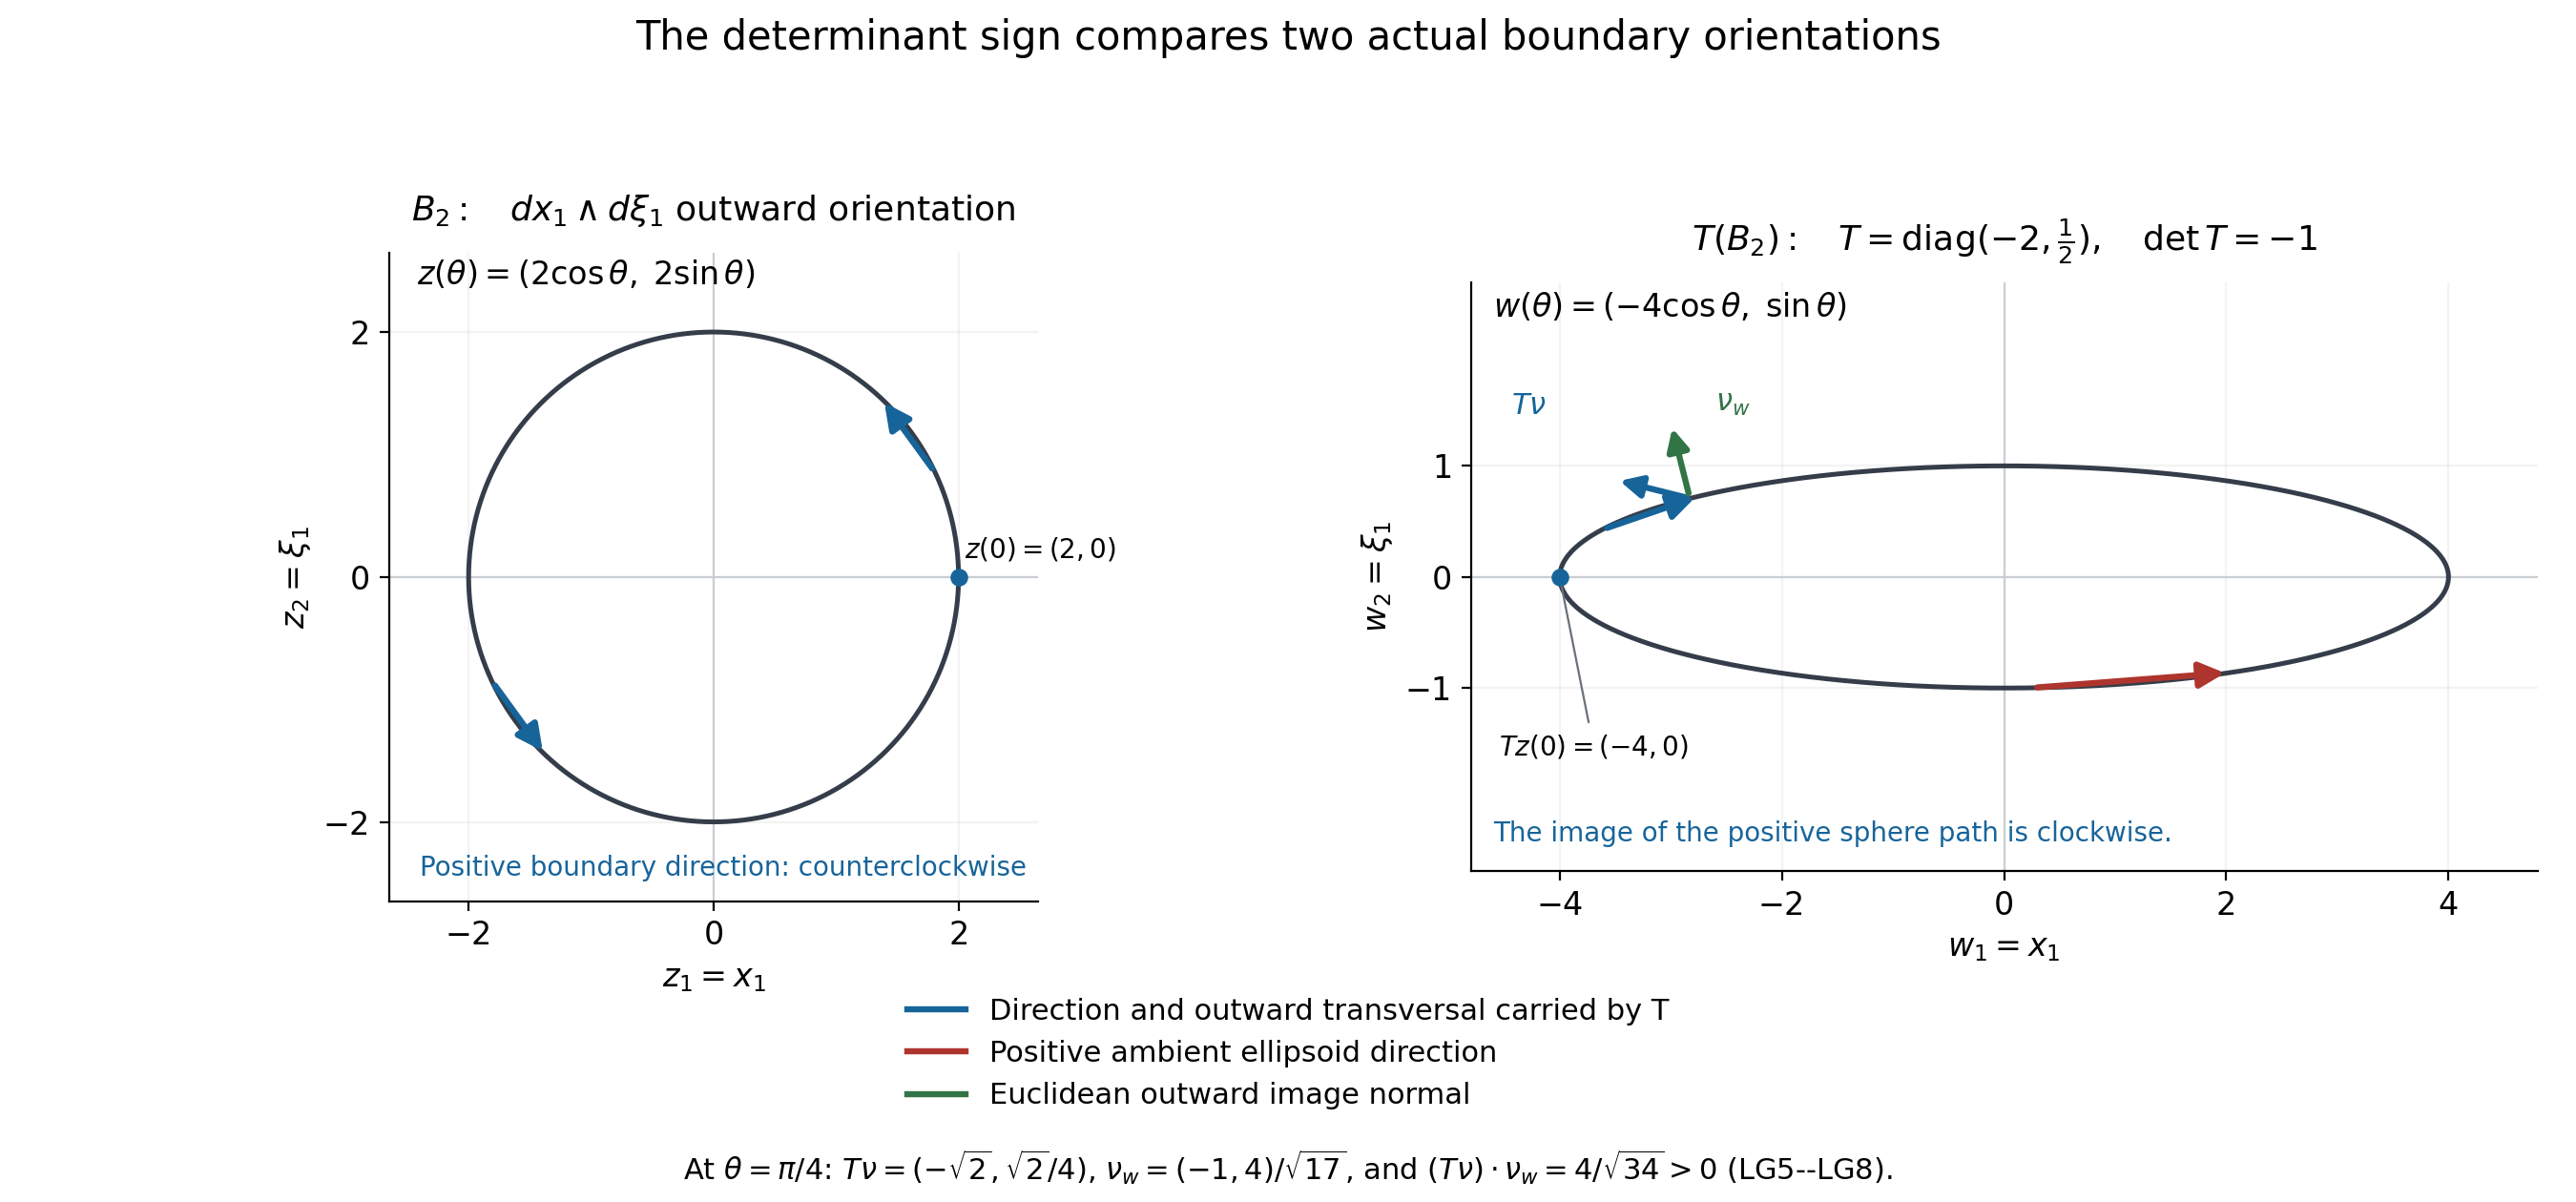
\includegraphics[keepaspectratio,alt={The original radius-two circle, its exact reflected and stretched ellipse, and both boundary orientations.}]{../figures/linear-phase-boundary-orientation-264.png}}
\caption{The original radius-two circle, its exact reflected and
stretched ellipse, and both boundary orientations.}
\end{figure}

\emph{The blue arrows carry the original positive input direction and
its outward transversal through the full map in (LO1). The red arrow
gives the positive ambient ellipse direction; the green arrow is its
Euclidean outward normal. The exact normal dot product and area
multiplier are (LO2), and their proof is (LG5)--(LG8). This auxiliary
geometric sample depicts no analytic index. Its reproducible
\href{../figures/linear-phase-boundary-orientation-264.py}{figure
source},
\href{../figures/linear-phase-boundary-orientation-264.svg}{vector
image} and
\href{../figures/linear-phase-boundary-orientation-264.json}{coordinate
record} retain every sample coordinate and factor.}

\subsection{14. Complete analytic receivers for the original
statements}\label{complete-analytic-receivers-for-the-original-statements}

The full flat matrix-index bridge has its complete finite proof in
\href{matrix-weyl-index-theorem.pdf}{the matrix-index lesson},
(LP3)--(LP14). Its (LP3) starts with the original two ordered errors and
a proved trace-norm remainder. Its (LP5)--(LP7) select the full
coordinate degree by the actual invertible paths and the finite Laurent
identity. Its (LP8)--(LP12) retain every intrinsic derivative and later
contraction, cancel repeated derivatives by the explicit
coordinate-label involution, and count every remaining ordered exterior
word. Therefore the same original finite calculation proves the direct
values used in Section5 here, independently of a cited algebraic index
theorem. The separate exterior-reduction lesson proves the same
calculation independently in (OE1)--(OE17). Its proof retains the full
ordered coefficients, coordinate selection, exterior multiplicities and
cutoff primitive.

In dimension one the finite choice is \(N=2\); in dimension two it is
\(N=4\). The entire finite coefficient is respectively the \(n=1\) and
\(n=2\) instance of the displayed (LP11), before its exact binomial and
factorial cancellation in (LP12). The proved cutoff primitive
(BN1)--(BN5) then gives, with the original outward orientation, \[
 D_1=-(-2\pi i)^{-1}{0!\over1!}={1\over2\pi i},\qquad
 D_2=-(-2\pi i)^{-2}{1!\over3!}={1\over24\pi^2}.
 \tag{LC1}
\] Applying those proved formulas to both original symbols \(a\) and
\(a\circ T\), whose full symbol and inverse bounds are (LT1)--(LT7), and
then using the complete original boundary comparison (LG1)--(LG11),
proves (LS8) and (LS9). For every dimension, the same argument uses the
full unchanged coefficient in (LS10), giving \[
\begin{aligned}
 \operatorname{ind}(a\circ T)^w
 &=D_n\int_{\partial B_R}^{\Omega}T^*\operatorname{Tr}(\theta_a^{2n-1})\\
 &=D_n{\det T\over|\det T|}
      \int_{\partial B_{R'}}^{\Omega}\operatorname{Tr}(\theta_a^{2n-1})\\
 &={\det T\over|\det T|}\operatorname{ind}a^w.
\end{aligned}
 \tag{LC2}
\] Here both original bounded Weyl operators have the actual same
Hilbert domain and target; each is Fredholm by IP14 and (LT1)--(LT7).
Both radii obey the full inequalities in (LG9). The complete beta moment
and its nonzero value were retained in (LG11) before division; the
determinant sign and the positive surface multiplier were proved in
(LG5)--(LG8). Thus this closes (LS10)--(LS11) without replacing any
original object or orientation. The complete reflected bounded example
(MI1)--(MI2) in the matrix-index lesson, with every denominator
derivative proved in its Section10.2, and the literal reciprocal
differential (LI2) here give the indices \(+1\) and \(-1\) in Section7.
The two exercise solutions then use only (LC2), (LC1), and the finite
graded matrix trace already proved in (EF1)--(EF4).

For the finite trace identity itself no matrix commutativity is assumed:
\(\operatorname{tr}(UV)=\sum_{j,k}U_{jk}V_{kj}=\sum_{k,j}V_{kj}U_{jk}=\operatorname{tr}(VU)\),
because these individual entries are scalars. Applied to each scalar
exterior component, its wedge permutation supplies precisely
\((-1)^{pq}\), proving (EF1); the \(2n-1\) cyclic one-form moves supply
the single minus in (EF2). All original ordered matrix products stay in
place before that trace operation. The finite local counterexample uses
the smooth cutoff constructed by the explicit scalar function in (LG1),
so it also has its stated compact support and all derivatives. Every
original claim, example and solution therefore has a proof here or in
the exact earlier programme lessons.

\end{document}
